% THIS IS AN EXAMPLE DOCUMENT FOR VLDB 2012
% based on ACM SIGPROC-SP.TEX VERSION 2.7
% Modified by  Gerald Weber <gerald@cs.auckland.ac.nz>
% Removed the requirement to include *bbl file in here. (AhmetSacan, Sep2012)
% Fixed the equation on page 3 to prevent line overflow. (AhmetSacan, Sep2012)

\documentclass{vldb}
\usepackage{graphicx}
\usepackage{balance}  % for  \balance command ON LAST PAGE  (only there!)


\begin{document}

% ****************** TITLE ****************************************

\title{Trusted SLA Guided Data Integration On Multi-Cloud Environments}

% possible, but not really needed or used for PVLDB:
%\subtitle{[Extended Abstract]
%\titlenote{A full version of this paper is available as\textit{Author's Guide to Preparing ACM SIG Proceedings Using \LaTeX$2_\epsilon$\ and BibTeX} at \texttt{www.acm.org/eaddress.htm}}}

% ****************** AUTHORS **************************************

% You need the command \numberofauthors to handle the 'placement
% and alignment' of the authors beneath the title.
%
% For aesthetic reasons, we recommend 'three authors at a time'
% i.e. three 'name/affiliation blocks' be placed beneath the title.
%
% NOTE: You are NOT restricted in how many 'rows' of
% "name/affiliations" may appear. We just ask that you restrict
% the number of 'columns' to three.
%
% Because of the available 'opening page real-estate'
% we ask you to refrain from putting more than six authors
% (two rows with three columns) beneath the article title.
% More than six makes the first-page appear very cluttered indeed.
%
% Use the \alignauthor commands to handle the names
% and affiliations for an 'aesthetic maximum' of six authors.
% Add names, affiliations, addresses for
% the seventh etc. author(s) as the argument for the
% \additionalauthors command.
% These 'additional authors' will be output/set for you
% without further effort on your part as the last section in
% the body of your article BEFORE References or any Appendices.

\numberofauthors{5} %  in this sample file, there are a *total*
% of EIGHT authors. SIX appear on the 'first-page' (for formatting
% reasons) and the remaining two appear in the \additionalauthors section.

\author{
% You can go ahead and credit any number of authors here,
% e.g. one 'row of three' or two rows (consisting of one row of three
% and a second row of one, two or three).
%
% The command \alignauthor (no curly braces needed) should
% precede each author name, affiliation/snail-mail address and
% e-mail address. Additionally, tag each line of
% affiliation/address with \affaddr, and tag the
% e-mail address with \email.
%
% 1st. author
\alignauthor 
Daniel A. S. Carvalho\\
       \affaddr{Universit\'e Jean Moulin Lyon 3}\\
       \affaddr{Centre de Recherche Magellan - IAE}\\
       \affaddr{Lyon, France}\\
       \email{first.last@univ-lyon3.fr}
% 2nd. author
\alignauthor 
Pl\'acido A. Souza Neto\\
       \affaddr{Federal Institute of Rio Grande do Norte}\\
       \affaddr{Natal, Brazil}\\
       \email{first.last@ifrn.edu.br}
% 3rd. author
\alignauthor Chirine Ghedira-Guegan\\
       \affaddr{Universit\'e Jean Moulin Lyon 3}\\
       \affaddr{Centre de Recherche Magellan - IAE}\\
       \affaddr{Lyon, France}\\
       \email{first.last@univ-lyon3.fr}
\and  % use '\and' if you need 'another row' of author names
% 4th. author
\alignauthor Nadia Bennani\\
       \affaddr{LIRIS - INSA}\\
       \affaddr{Lyon, France}\\
       \email{first.last@insa-lyon.fr}
% 5th. author
\alignauthor Genoveva Vargas-Solar\\
       \affaddr{CNRS-LIG}\\
       \affaddr{Grenoble, France}
       \email{first.last@imag.fr}
}
% There's nothing stopping you putting the seventh, eighth, etc.
% author on the opening page (as the 'third row') but we ask,
% for aesthetic reasons that you place these 'additional authors'
% in the \additional authors block, viz.
%\date{30 July 1999}
% Just remember to make sure that the TOTAL number of authors
% is the number that will appear on the first page PLUS the
% number that will appear in the \additionalauthors section.


\maketitle

\begin{abstract}
\ldots
\end{abstract}


\section{Introduction}

\section{Related works}
Maybe merge this section while introducing...

\section{General Approach}
\begin{figure}[h!]
\centering
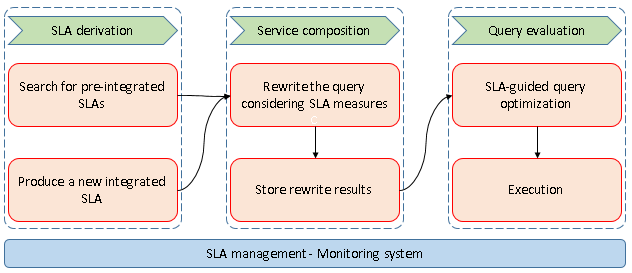
\includegraphics[scale=0.5]{general_approach}
\caption{A sample black and white graphic (.pdf format).}
\label{fig:generalapproach}
\end{figure}

\section{Data integration model}


\section{Preliminary results}


\section{Conclusions}


%\end{document}  % This is where a 'short' article might terminate

% ensure same length columns on last page (might need two sub-sequent latex runs)

%ACKNOWLEDGMENTS are optional
\section{Acknowledgments}
ACKNOWLEDGMENTS are optional...

% The following two commands are all you need in the
% initial runs of your .tex file to
% produce the bibliography for the citations in your paper.
\bibliographystyle{abbrv}

\bibliography{vldb_sample}  
% vldb_sample.bib is the name of the Bibliography in this case
% You must have a proper ".bib" file
%  and remember to run:
% latex bibtex latex latex
% to resolve all references
 
\end{document}
